\documentclass[margin,line]{res}
\usepackage{graphicx}
\usepackage[cm]{fullpage}
\usepackage{hyperref}
\usepackage{url}
\urlstyle{same} 

\usepackage[utf8]{inputenc}
\usepackage[T1]{fontenc}

\oddsidemargin -.5in
\evensidemargin -.5in
\textwidth=6.0in
\itemsep=0in
\parsep=0in

\newenvironment{list1}{
  \begin{list}{\ding{113}}{%
      \setlength{\itemsep}{0in}
      \setlength{\parsep}{0in} \setlength{\parskip}{0in}
      \setlength{\topsep}{0in} \setlength{\partopsep}{0in} 
      \setlength{\leftmargin}{0.17in}}}{\end{list}}
\newenvironment{list2}{
  \begin{list}{$\bullet$}{%
      \setlength{\itemsep}{0in}
      \setlength{\parsep}{0in} \setlength{\parskip}{0in}
      \setlength{\topsep}{0in} \setlength{\partopsep}{0in} 
      \setlength{\leftmargin}{0.2in}}}{\end{list}}

\begin{document}

\name{
\begin{tabular*}{7.4in} {@{\extracolsep{\fill}}lr}
Toby Dylan Hocking & Curriculum Vitae 
\end{tabular*}
}

\begin{resume}
\section{\sc Contact and General Info}
\vspace{.05in}
\begin{tabular*}{6.1in} {@{\extracolsep{\fill}}ll}
 NAU Building 90, Office 210 & Birth: 17 March 1984 in Newport Beach, California\\
 1295 S. Knoles Dr.  & Citizenship: USA. \\            
  Flagstaff, AZ 86011 & Languages: English (native), French
                        (fluent since 2009). \\
  E-mail:  toby.hocking@nau.edu & Web: \url{http://tdhock.github.io}, \href{https://tdhock.github.io/blog/2022/erdos-number/}{Erd\H{o}s number = 3}. \\
\end{tabular*}

\section{\sc Research Interests}

Machine learning algorithms, statistical software, and data
visualization techniques. Emphasis on efficient algorithms for large
datasets, based on constrained optimization (regression,
classification, ranking, clustering, segmentation, changepoint
detection, survival analysis). Application domains include medicine,
genomics, neuroscience, recommendation systems, image and text analysis.

\section{\sc Professional Experience \\ \hspace{0.1cm} \\ 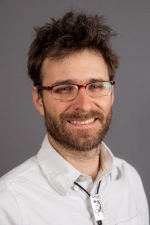
\includegraphics[width=3cm]{HOCKING-rectangle-lores.jpg}}

{\bf Northern Arizona University}, Flagstaff, Arizona, USA (2018-present).\\
\vspace*{-.1in}
\begin{list2}
\item[] Tenure-Track Assistant Professor, School of Informatics, Computing, and Cyber Systems.
\item[] ``Optimization algorithms for machine learning and interactive data analysis.''
\end{list2}

{\bf McGill University}, Montreal, Canada (2014-2018).\\
\vspace*{-.1in}
\begin{list2}
\item[] Postdoc with Guillaume Bourque, Department of Human Genetics.
\item[]``Changepoint detection and regression models for peak detection in genomic data.''
\end{list2}

{\bf Tokyo Institute of Technology}, Tokyo, Japan (2013).\\
\vspace*{-.1in}
\begin{list2}
\item[] Postdoc with Masashi Sugiyama, Department of Computer Science.
\item[] ``Support vector machines for ranking and comparing.''
\end{list2}

{\bf Sangamo BioSciences}, Richmond, CA, USA (2006-2008).\\
\vspace*{-.1in}
\begin{list2}
\item[] Research Assistant with Jeff Miller in the Zinc Finger Technology group.
\item[] ``A web app for visualization and statistical analysis of experimental data.''
\end{list2}

\section{\sc Education}

{\bf \'{E}cole Normale Sup\'{e}rieure}, Cachan, France (2009-2012).\\
\vspace*{-.1in}
\begin{list2}
\item[] Math Ph.D. with Francis Bach, D\'{e}partement d'Informatique; Jean-Philippe Vert, Institut Curie.
\item[] ``Learning algorithms and statistical software, with applications to bioinformatics."
\end{list2}

{\bf Universit\'e Paris 6}, Paris, France (2008-2009).\\
\vspace*{-.1in}
\begin{list2}
\item[] Master of Statistics, internship at INRA with Mathieu Gautier and Jean-Louis Foulley.
\item[] ``A Bayesian Outlier Criterion to Detect SNPs under Selection in Large Data Sets."
\end{list2}

{\bf University of California, Berkeley}, CA, USA (2002-2006).\\
\vspace*{-.1in}
\begin{list2}
\item[] Double B.A. in Statistics, Molecular and Cell Biology; thesis in Statistics with Terry Speed.
\item[] ``Chromosomal copy number analysis using SNP microarrays and a binomial test statistic.'' 
\end{list2}

\section{\sc Honors and Awards (Selected)}

Co-PI on National Science Foundation grant, \$3,000,000, Sept 2021 to
Aug 2026. ``MIM: Discovering in reverse – using isotopic translation
of omics to reveal ecological interactions in microbiomes.'' Role:
supervise PHD student working on machine learning analysis of new
metabolic flux data, in order to infer new types of interactions
between microbes.

Senior personnel on NAU sub-contract of Department of Energy grant,
\$9,000,000, 2022-2024, Lawrence Livermore National Laboratory
Science Focus Area program entitled ``Microbes Persist: Systems
Biology of the Soil Microbiome'' led by PI Jennifer
Pett-Ridge. Role: machine learning analysis of microbiome
interaction networks, identifying taxa and traits that are associated
with soil carbon cycling processes.

Senior personnel on Missouri Department of Elementary and Secondary
Education grant, \$1,509,570, July 2021--June 2022, contract entitled
``MMD-DCI Research, Development, \& Leadership'' led by PI Ronda
Jenson. Role: summer salary and mentoring two graduate students on
interpretable machine learning algorithms for Predictive Modeling
Framework for District Continuous Improvement.

Air Force Research Laboratory, Summer Faculty Fellowship, May--July
2021, ``Machine learning algorithms for understanding physically
unclonable functions based on resistive memory devices.''

PI on R Consortium Grant, \$34,000, Jan--Dec 2020, ``RcppDeepState: an easy
way to fuzz test compiled code in R packages.''

``Mobilit\'e entrant'' travel award to do research with Guillem Rigaill in
Universit\'e Evry, France, 2016.

International useR conference, Best Student Poster Award, ``Adding
direct labels to plots,'' 2011.

INRIA/INRA (French computer science and agricultural research institutes), Ph.D. scholarship, 2009 (declined).

UC Berkeley, Department of Statistics VIGRE research scholarship, 2001.

%UC Berkeley, Cal Band George Miller scholarship, 2000.

\section{\sc Papers in progress and under review}

Tao F, Huang Y, Hungate BA, Manzoni S, Frey SD, Schmidt MWI,
Reichstein M, Carvalhais N, Ciais P, Jiang L, Lehmann J, Mishra U,
Hugelius G, {\bf Hocking TD}, Lu X, Shi Z, Viatkin K, Vargas R, Yigini
Y, Omuto C, Malik AA, Peralta G, Cuevas-Corona R, Di Paolo LE, Luotto
I, Liao C, Liang YS, Saynes VS, Huang X, Luo Y. Microbial carbon use
efficiency promoting global soil carbon storage. Under review in {\it
  Nature}.

Hillman J, {\bf Hocking TD}. Optimizing ROC Curves with a Sort-Based
Surrogate Loss Function for Binary Classification and Changepoint
Detection. Under review in {\it Journal of Machine Learning Research}.

Runge V, {\bf Hocking TD}, Romano G, Afghah F, Fearnhead P, Rigaill
G. gfpop: an R Package for Univariate Graph-Constrained Change-point
Detection. Under review in {\it Journal of Statistical Software},
arXiv:2002.03646.

Venuto D, {\bf Hocking TD}, Spanurattana S, Sugiyama M. Support vector
comparison machines. Under review in {\it Machine Learning},
arXiv:1401.8008.

Barnwal A, Cho H, {\bf Hocking TD}. Survival regression with
accelerated failure time model in XGBoost. Accepted in {\it Journal of
  Computational and Graphical Statistics}.

{\bf Hocking TD}, Srivastava A. Labeled Optimal Partitioning. Accepted
in {\it Computational Statistics}.

\section{\sc Peer-reviewed journal papers}

{\bf Hocking TD}, Rigaill G, Fearnhead P, Bourque G. Generalized
Functional Pruning Optimal Partitioning (GFPOP) for Constrained
Changepoint Detection in Genomic Data. {\it Journal of Statistical
  Software}, Vol. 101, Issue 10 (2022).

Chaves AP, Egbert J, {\bf Hocking TD}, Doerry E, Gerosa MA. Chatbots
language design: the influence of language use on user
experience. {\it ACM Transactions on Computer-Human Interaction} 29,
2, Article 13 (2022).

{\bf Hocking TD}, Vargovich J. Linear Time Dynamic Programming for
Computing Breakpoints in the Regularization Path of Models Selected
From a Finite Set. {\it Journal of Computational and Graphical
  Statistics} (2021), doi:10.1080/10618600.2021.2000422.

{\bf Hocking TD}. Wide-to-tall data reshaping using regular
expressions and the nc package. {\it R Journal} (2021),
doi:10.32614/RJ-2021-029.

Liehrmann A, Rigaill G, {\bf Hocking TD}. Increased peak detection
accuracy in over-dispersed ChIP-seq data with supervised segmentation
models. {\it BMC Bioinformatics} 22, Article number: 323 (2021).

Fotoohinasab A, {\bf Hocking TD}, Afghah F. A Greedy Graph Search
Algorithm Based on Changepoint Analysis for Automatic QRS-Complex
Detection. {\it Computers in Biology and Medicine} 130 (2021).

Abraham A, Prys-Jones T, De Cuyper A, Ridenour C, Hempson G, {\bf
  Hocking TD}, Clauss M, Doughty C. Improved estimation of gut passage
time considerably affects trait-based dispersal models. {\it
  Functional Ecology} (2021); 35: 860-869.

{\bf Hocking TD}, Rigaill G, Fearnhead P, Bourque G. Constrained
dynamic programming and supervised penalty learning algorithms for
peak detection in genomic data. {\it Journal of Machine Learning
  Research} 21(87):1--40, (2020).

{\bf Hocking TD}. Comparing namedCapture with other R packages for
regular expressions. {\it R Journal} (2019). doi:10.32614/RJ-2019-050

Jewell S, {\bf Hocking TD}, Fearnhead P, Witten D. Fast Nonconvex
Deconvolution of Calcium Imaging Data. {\it Biostatistics} (2019), doi:
10.1093/biostatistics/kxy083.

Depuydt P, Koster J, Boeva V, {\bf Hocking TD}, Speleman F,
Schleiermacher G, De Preter K. Meta-mining of copy number profiles of
high-risk neuroblastoma tumors. {\it Scientific Data} (2018).

Alirezaie N, Kernohan KD, Hartley T, Majewski J, {\bf Hocking
  TD}. ClinPred: Prediction Tool to Identify Disease-Relevant
Nonsynonymous Single-Nucleotide Variants. American Journal of Human
Genetics (2018). doi:10.1016/j.ajhg.2018.08.005

Sievert C, Cai J, VanderPlas S, Khan F, Ferris K, {\bf Hocking
  TD}. Extending ggplot2 for linked and dynamic web graphics. {\it
  Journal of Computational and Graphical Statistics} (2018).

Depuydt P, Boeva V, {\bf Hocking TD}, {\it et al}. Genomic
Amplifications and Distal 6q Loss: Novel Markers for Poor Survival in
High-risk Neuroblastoma Patients. {\it Journal of the National Cancer
  Institute} (2018). DOI:10.1093/jnci/djy022.

{\bf Hocking TD}, Goerner-Potvin P, Morin A, Shao X, Pastinen T,
Bourque G. Optimizing ChIP-seq peak detectors using visual labels and
supervised machine learning. {\it Bioinformatics} (2017) 33 (4): 491-499.

Shimada K, Shimada S, Sugimoto K, Nakatochi M, Suguro M, Hirakawa A,
{\bf Hocking TD}, Takeuchi I, Tokunaga T, Takagi Y, Sakamoto A, Aoki T, Naoe
T, Nakamura S, Hayakawa F, Seto M, Tomita A, Kiyoi H. Development and
analysis of patient-derived xenograft mouse models in intravascular
large B-cell lymphoma. {\it Leukemia} (2016).

Chicard M, Boyault S, Colmet-Daage L, Richer W, Gentien D, Pierron G,
Lapouble E, Bellini A, Clement N, Iacono I, Bréjon S, Carrere M, Reyes
C, {\bf Hocking TD}, Bernard V, Peuchmaur M, Corradini N, Faure-Conter
C, Coze C, Plantaz D, Defachelles A-S, Thebaud E, Gambart M, Millot F,
Valteau-Couanet D, Michon J, Puisieux A, Delattre O, Combaret V,
Schleiermacher G. Genomic copy number profiling using circulating free
tumor DNA highlights heterogeneity in neuroblastoma. {\it Clinical Cancer
Research} (2016).

Maidstone R, {\bf Hocking TD}, Rigaill G, Fearnhead P. On optimal
multiple changepoint algorithms for large data. {\it Statistics and
Computing} (2016). doi:10.1007/s11222-016-9636-3 

Suguro M, Yoshida N, Umino A, Kato H, Tagawa H, Nakagawa M, Fukuhara
N, Karnan S, Takeuchi I, {\bf Hocking TD}, Arita K, Karube K, Tsuzuki
S, Nakamura S, Kinoshita T, Seto M. Clonal heterogeneity of lymphoid
malignancies correlates with poor prognosis. {\it Cancer Sci.} (2014)
Jul;105(7):897-904.

{\bf Hocking TD}, Boeva V, Rigaill G, Schleiermacher G,
Janoueix-Lerosey I, Delattre O, Richer W, Bourdeaut F, Suguro M, Seto
M, Bach F, Vert J-P. SegAnnDB: interactive Web-based genomic
segmentation. {\it Bioinformatics} (2014) 30 (11):
1539-1546. DOI:10.1093/bioinformatics/btu072

{\bf Hocking TD}, Wutzler T, Ponting K and Grosjean P. Sustainable,
extensible documentation generation using inlinedocs. {\it Journal of
Statistical Software} (2013), 54(6), 1-20. DOI:10.18637/jss.v054.i06

{\bf Hocking TD}, Schleiermacher G, Janoueix-Lerosey I, Boeva V, Cappo
J, Delattre O, Bach F, Vert J-P. Learning smoothing models of copy
number profiles using breakpoint annotations. {\it BMC Bioinfo.} (2013),
14:164. DOI:10.1186/1471-2105-14-164

Gautier M, {\bf Hocking TD}, Foulley JL. A Bayesian outlier criterion
to detect SNPs under selection in large data sets. {\it PloS ONE} 5
(8), e11913 (2010).

Doyon Y, McCammon JM, Miller JC, Faraji F, Ngo C, Katibah GE, Amora R,
{\bf Hocking TD}, Zhang L, Rebar EJ, Gregory PD, Urnov FD, Amacher
SL. Heritable targeted gene disruption in zebrafish using designed
zinc-finger nucleases. {\it Nature biotechnology} 26 (6), 702-70
(2008).

\section{\sc Peer-reviewed conference papers}

In addition to peer-reviewed journals, I publish papers at
highly competitive computer science conferences like {\it ICML} and {\it NeurIPS}, with
double-blind peer reviews, and $\approx$20\% acceptance rates.

Kolla AC, Groce A, {\bf Hocking TD}. Fuzz Testing the Compiled Code in
R Packages. IEEE 32nd International Symposium on Software
Reliability Engineering (ISSRE 2021), pp. 300-308, doi:
10.1109/ISSRE52982.2021.00040.

Fotoohinasab A, {\bf Hocking TD}, Afghah F. A Graph-Constrained
Changepoint Learning Approach for Automatic QRS-Complex
Detection. {\it Asilomar Conference on Signals, Systems, and
  Computers} (2020).

Fotoohinasab A, {\bf Hocking TD}, Afghah F. A Graph-constrained
Changepoint Detection Approach for ECG Segmentation. 
{\it 42th Annual International Conference of the IEEE Engineering in
  Medicine and Biology Society (EMBC 2020)}.

{\bf Hocking TD}, Bourque G. Machine Learning Algorithms for
Simultaneous Supervised Detection of Peaks in Multiple Samples and
Cell Types. {\it Pacific Symposium on Biocomputing} 25:367-378 (2020).

Drouin A, {\bf Hocking TD}, Laviolette F. Maximum margin interval
trees. {\it Neural Information Processing Systems (NeurIPS)}, 2017.

{\bf Hocking TD}, Rigaill G, Bourque G. PeakSeg: constrained optimal
segmentation and supervised penalty learning for peak detection in
count data. {\it International Conference on Machine Learning (ICML)},
2015.

{\bf Hocking TD}, Rigaill G, Bach F, Vert J-P. Learning sparse
penalties for change-point detection using max-margin interval
regression. {\it International Conference on Machine Learning (ICML)}, 2013.

{\bf Hocking TD}, Joulin A, Bach F, Vert J-P. Clusterpath: an
Algorithm for Clustering using Convex Fusion Penalties. {\it International Conference on Machine Learning (ICML)}, 2011.

\section{\sc Books, Chapters, Manuals}

{\bf Hocking TD} and Killick R. {\it Changepoint detection algorithms
  and applications in R}. Textbook in preparation.

{\bf Hocking TD}. Introduction to Machine Learning and Neural
Networks. Chapter in textbook {\it Land Carbon Cycle Modeling: Matrix
  Approach, Data Assimilation, and Ecological Forecasting} edited by
Yiqi Luo. (expected publication Jan 2022)

{\bf Hocking TD}. Animated interactive data visualization using the
grammar of graphics (The animint2 Manual), 17 web pages/chapters with
interactive graphics and exercises. (2018)

\section{\sc Conference Tutorials}

{\bf Hocking TD}, Killick R. Introduction to optimal changepoint
detection algorithms, {\it useR} 2017.

{\bf Hocking TD}, Ekstr\o m CT. Understanding and creating interactive
graphics, {\it useR} 2016.

\section{\sc Invited talks (selected)}

Keynote for IEEE conference in Prescott Arizona, University of Arizona
Math/Stats seminar (2022); ASU West ML Day,
\href{https://arizona.hosted.panopto.com/Panopto/Pages/Viewer.aspx?id=4e87c8d0-96d2-40d1-808c-ad16014c6962}{TRIPODS
  University of Arizona}, IEEE NJACS (2021); NAU Math Department
Colloquium (2018); University of Waterloo, Université de Montréal,
Sainte-Justine Children's Hospital, University of Québec à Montréal,
Polytechnique Montréal (2017); Universit\'e Laval Centre for Big Data
Research (2016); McGill Barbados epigenomics workshop (2015); Sapporo
Japan Workshop on Machine Learning and Applications to Biology (2013);
Google Research New York, Universit\'e Rennes, Universit\'e Angers,
INRIA Lille (2012); Institut de Biologie de Lille (2011).

\section{\sc Consulting (selected)}

Acronis SCS, cybersecurity company in Phoenix (2022). Interpretable
and non-linear machine learning algorithms which use source code
analysis to predict software vulnerabilities.

Plotly, data visualization startup in Montreal (2015). Original author
of ggplot functionality in plotly R package.

\section{\sc Teaching}

All of my course materials are freely available online,
\url{https://tdhock.github.io/teaching/}

Spring 2022, Northern Arizona University, CS570, Deep Learning.

Fall 2021, Northern Arizona University, CS499/599, Unsupervised Learning.

Summer 2021, 60 minute lecture ``Introduction to Machine Learning and
Neural Networks'' for summer school on ``New Advances in Land Carbon
Cycle Modeling.''

Spring 2021, Northern Arizona University, CS470, Artificial Intelligence.

Fall 2020, Northern Arizona University, CS499/599, Unsupervised
Learning.

Summer 2020, 90 minute lecture ``Introduction to Machine Learning and
Neural Networks'' for summer school on ``New Advances in Land Carbon
Cycle Modeling.''

Spring 2020, Northern Arizona University, CS499, Deep Learning.

Fall 2019, Northern Arizona University, CS/EE599, Reproducible Machine
Learning Research.

Spring 2019, Northern Arizona University, CS499, Optimization
algorithms for machine learning.

\section{\sc Professional Service}

2022, Member of steering committee for R project in Google Season of Docs.

2021--present, machine learning editor for rOpenSci Statistical Software.

2018--present, editor for Journal of Statistical Software.

2021--present, co-author of
\href{https://contributor.r-project.org/rdevguide/}{R Development
  Guide} and member of R Contribution Working Group (resources for
making it easy/accessible to contribute improvements to base R).

2012--present, co-administrator and mentor for R project in Google
Summer of Code (teaching how to create and improve R packages).

2017--2018, president of organizing committee for ``R in Montreal
2018'' conference.

2010--present: peer reviewer for Technometrics, International
Conference on Machine Learning (ICML), Advances in Neural Information
Processing Systems (NeurIPS), Journal of Machine Learning Research
(JMLR), Artificial Intelligence Review, Journal of Computational and
Graphical Statistics (JCGS), R Journal, Bioinformatics, PLOS
Computational Biology, BMC Bioinformatics, IEEE Transactions on
Pattern Analysis and Machine Intelligence, Information and Inference,
Journal of Statistical Computation and Simulation, Computo, Genome
Biology.

\section{\sc Software Online (Selected)} 

Numerous free/open-source software contributions using R, C, C++,
Python, and JavaScript.

{\bf R}: contributions to base R regex functionalty and data reshaping
in data.table package. Maintainer of numerous R packages (17 on CRAN
as of Feb 2022) for machine learning (changepoint detection,
classification, regression, ranking, etc), directlabels for labeled
figures, animint2 for animated interactive figures, inlinedocs for
documentation generation.

{\bf Python}: contributions to pandas module for data manipulation
(str.extractall regex functionality), maintainer of GUI/web server
software for labeling and changepoint detection in genomic data
(annotate\_regions, SegAnnDB, PeakLearner).

\section{\sc References}

\noindent {\bf Yiqi Luo}, collaborator on research and teaching (summer school, textbook).\\
Regents' Professor, Department of Biological Sciences, Northern Arizona University\\
Phone: +1 (928) 523-1925, E-mail: yiqi.luo@nau.edu\\
Web: \url{https://www2.nau.edu/luo-lab/?member_info&id=52}

\noindent {\bf Eck Doerry}, collaborator on research and familiar with my teaching.\\
Professor, School of Informatics, Computing and Cyber Systems, Northern Arizona University\\
Phone: +1 (928) 523-9377, E-mail: Eck.Doerry@nau.edu, Web: \url{https://www.cefns.nau.edu/~edo}

\noindent {\bf Jarrett ``Jay'' Barber}, colleague familiar with my teaching.\\
Associate Professor, School of Informatics, Computing and Cyber Systems,\\
Northern Arizona University, 
Phone: +1 (928) 523-6869, E-mail: Jarrett.Barber@nau.edu

\noindent {\bf Alex Groce}, collaborator on research papers and grants.\\
Associate Professor, School of Informatics, Computing and Cyber Systems,\\
Northern Arizona University, 
Phone: +1 (928) 523-8263, E-mail: Alex.Groce@nau.edu

\noindent {\bf Fatemeh Afghah}, collaborator on research papers and grants.\\
Associate Professor, Clemson University, Phone: +1 (864) 656-0100, E-mail: fafghah@clemson.edu, Web: \url{https://fafghah.people.clemson.edu/}

\noindent {\bf Guillem Rigaill}, collaborator on research papers and grants.\\
Researcher at INRAE (French Agronomy Research Institute)\\
Phone: +33 (0) 1 64 85 35 44, E-mail: guillem.rigaill@inrae.fr\\
Web: \url{http://www.math-evry.cnrs.fr/members/Grigaill/welcome}

\end{resume}
\end{document}




